\documentclass[1p]{elsarticle_modified}
%\bibliographystyle{elsarticle-num}

%\usepackage[colorlinks]{hyperref}
%\usepackage{abbrmath_seonhwa} %\Abb, \Ascr, \Acal ,\Abf, \Afrak
\usepackage{amsfonts}
\usepackage{amssymb}
\usepackage{amsmath}
\usepackage{amsthm}
\usepackage{scalefnt}
\usepackage{amsbsy}
\usepackage{kotex}
\usepackage{caption}
\usepackage{subfig}
\usepackage{color}
\usepackage{graphicx}
\usepackage{xcolor} %% white, black, red, green, blue, cyan, magenta, yellow
\usepackage{float}
\usepackage{setspace}
\usepackage{hyperref}

\usepackage{tikz}
\usetikzlibrary{arrows}

\usepackage{multirow}
\usepackage{array} % fixed length table
\usepackage{hhline}

%%%%%%%%%%%%%%%%%%%%%
\makeatletter
\renewcommand*\env@matrix[1][\arraystretch]{%
	\edef\arraystretch{#1}%
	\hskip -\arraycolsep
	\let\@ifnextchar\new@ifnextchar
	\array{*\c@MaxMatrixCols c}}
\makeatother %https://tex.stackexchange.com/questions/14071/how-can-i-increase-the-line-spacing-in-a-matrix
%%%%%%%%%%%%%%%

\usepackage[normalem]{ulem}

\newcommand{\msout}[1]{\ifmmode\text{\sout{\ensuremath{#1}}}\else\sout{#1}\fi}
%SOURCE: \msout is \stkout macro in https://tex.stackexchange.com/questions/20609/strikeout-in-math-mode

\newcommand{\cancel}[1]{
	\ifmmode
	{\color{red}\msout{#1}}
	\else
	{\color{red}\sout{#1}}
	\fi
}

\newcommand{\add}[1]{
	{\color{blue}\uwave{#1}}
}

\newcommand{\replace}[2]{
	\ifmmode
	{\color{red}\msout{#1}}{\color{blue}\uwave{#2}}
	\else
	{\color{red}\sout{#1}}{\color{blue}\uwave{#2}}
	\fi
}

\newcommand{\Sol}{\mathcal{S}} %segment
\newcommand{\D}{D} %diagram
\newcommand{\A}{\mathcal{A}} %arc


%%%%%%%%%%%%%%%%%%%%%%%%%%%%%5 test

\def\sl{\operatorname{\textup{SL}}(2,\Cbb)}
\def\psl{\operatorname{\textup{PSL}}(2,\Cbb)}
\def\quan{\mkern 1mu \triangleright \mkern 1mu}

\theoremstyle{definition}
\newtheorem{thm}{Theorem}[section]
\newtheorem{prop}[thm]{Proposition}
\newtheorem{lem}[thm]{Lemma}
\newtheorem{ques}[thm]{Question}
\newtheorem{cor}[thm]{Corollary}
\newtheorem{defn}[thm]{Definition}
\newtheorem{exam}[thm]{Example}
\newtheorem{rmk}[thm]{Remark}
\newtheorem{alg}[thm]{Algorithm}

\newcommand{\I}{\sqrt{-1}}
\begin{document}

%\begin{frontmatter}
%
%\title{Boundary parabolic representations of knots up to 8 crossings}
%
%%% Group authors per affiliation:
%\author{Yunhi Cho} 
%\address{Department of Mathematics, University of Seoul, Seoul, Korea}
%\ead{yhcho@uos.ac.kr}
%
%
%\author{Seonhwa Kim} %\fnref{s_kim}}
%\address{Center for Geometry and Physics, Institute for Basic Science, Pohang, 37673, Korea}
%\ead{ryeona17@ibs.re.kr}
%
%\author{Hyuk Kim}
%\address{Department of Mathematical Sciences, Seoul National University, Seoul 08826, Korea}
%\ead{hyukkim@snu.ac.kr}
%
%\author{Seokbeom Yoon}
%\address{Department of Mathematical Sciences, Seoul National University, Seoul, 08826,  Korea}
%\ead{sbyoon15@snu.ac.kr}
%
%\begin{abstract}
%We find all boundary parabolic representation of knots up to 8 crossings.
%
%\end{abstract}
%\begin{keyword}
%    \MSC[2010] 57M25 
%\end{keyword}
%
%\end{frontmatter}

%\linenumbers
%\tableofcontents
%
\newcommand\colored[1]{\textcolor{white}{\rule[-0.35ex]{0.8em}{1.4ex}}\kern-0.8em\color{red} #1}%
%\newcommand\colored[1]{\textcolor{white}{ #1}\kern-2.17ex	\textcolor{white}{ #1}\kern-1.81ex	\textcolor{white}{ #1}\kern-2.15ex\color{red}#1	}

{\Large $\underline{12a_{0636}~(K12a_{0636})}$}

\setlength{\tabcolsep}{10pt}
\renewcommand{\arraystretch}{1.6}
\vspace{1cm}\begin{tabular}{m{100pt}>{\centering\arraybackslash}m{274pt}}
\multirow{5}{120pt}{
	\centering
	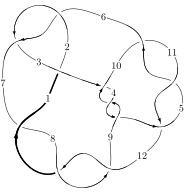
\includegraphics[width=112pt]{../../../GIT/diagram.site/Diagrams/png/1437_12a_0636.png}\\
\ \ \ A knot diagram\footnotemark}&
\allowdisplaybreaks
\textbf{Linearized knot diagam} \\
\cline{2-2}
 &
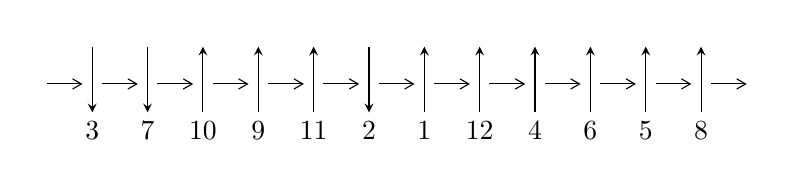
\begin{tikzpicture}[x=20pt, y=17pt]
	% nodes
	\node (C0) at (0, 0) {};
	\node (C1) at (1, 0) {};
	\node (C1U) at (1, +1) {};
	\node (C1D) at (1, -1) {3};

	\node (C2) at (2, 0) {};
	\node (C2U) at (2, +1) {};
	\node (C2D) at (2, -1) {7};

	\node (C3) at (3, 0) {};
	\node (C3U) at (3, +1) {};
	\node (C3D) at (3, -1) {10};

	\node (C4) at (4, 0) {};
	\node (C4U) at (4, +1) {};
	\node (C4D) at (4, -1) {9};

	\node (C5) at (5, 0) {};
	\node (C5U) at (5, +1) {};
	\node (C5D) at (5, -1) {11};

	\node (C6) at (6, 0) {};
	\node (C6U) at (6, +1) {};
	\node (C6D) at (6, -1) {2};

	\node (C7) at (7, 0) {};
	\node (C7U) at (7, +1) {};
	\node (C7D) at (7, -1) {1};

	\node (C8) at (8, 0) {};
	\node (C8U) at (8, +1) {};
	\node (C8D) at (8, -1) {12};

	\node (C9) at (9, 0) {};
	\node (C9U) at (9, +1) {};
	\node (C9D) at (9, -1) {4};

	\node (C10) at (10, 0) {};
	\node (C10U) at (10, +1) {};
	\node (C10D) at (10, -1) {6};

	\node (C11) at (11, 0) {};
	\node (C11U) at (11, +1) {};
	\node (C11D) at (11, -1) {5};

	\node (C12) at (12, 0) {};
	\node (C12U) at (12, +1) {};
	\node (C12D) at (12, -1) {8};
	\node (C13) at (13, 0) {};

	% arrows
	\draw[->,>={angle 60}]
	(C0) edge (C1) (C1) edge (C2) (C2) edge (C3) (C3) edge (C4) (C4) edge (C5) (C5) edge (C6) (C6) edge (C7) (C7) edge (C8) (C8) edge (C9) (C9) edge (C10) (C10) edge (C11) (C11) edge (C12) (C12) edge (C13) ;	\draw[->,>=stealth]
	(C1U) edge (C1D) (C2U) edge (C2D) (C3D) edge (C3U) (C4D) edge (C4U) (C5D) edge (C5U) (C6U) edge (C6D) (C7D) edge (C7U) (C8D) edge (C8U) (C9D) edge (C9U) (C10D) edge (C10U) (C11D) edge (C11U) (C12D) edge (C12U) ;
	\end{tikzpicture} \\
\hhline{~~} \\& 
\textbf{Solving Sequence} \\ \cline{2-2} 
 &
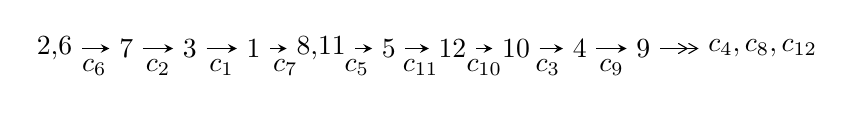
\begin{tikzpicture}[x=23pt, y=7pt]
	% node
	\node (A0) at (-1/8, 0) {2,6};
	\node (A1) at (1, 0) {7};
	\node (A2) at (2, 0) {3};
	\node (A3) at (3, 0) {1};
	\node (A4) at (65/16, 0) {8,11};
	\node (A5) at (41/8, 0) {5};
	\node (A6) at (49/8, 0) {12};
	\node (A7) at (57/8, 0) {10};
	\node (A8) at (65/8, 0) {4};
	\node (A9) at (73/8, 0) {9};
	\node (C1) at (1/2, -1) {$c_{6}$};
	\node (C2) at (3/2, -1) {$c_{2}$};
	\node (C3) at (5/2, -1) {$c_{1}$};
	\node (C4) at (7/2, -1) {$c_{7}$};
	\node (C5) at (37/8, -1) {$c_{5}$};
	\node (C6) at (45/8, -1) {$c_{11}$};
	\node (C7) at (53/8, -1) {$c_{10}$};
	\node (C8) at (61/8, -1) {$c_{3}$};
	\node (C9) at (69/8, -1) {$c_{9}$};
	\node (A10) at (11, 0) {$c_{4},c_{8},c_{12}$};

	% edge
	\draw[->,>=stealth]	
	(A0) edge (A1) (A1) edge (A2) (A2) edge (A3) (A3) edge (A4) (A4) edge (A5) (A5) edge (A6) (A6) edge (A7) (A7) edge (A8) (A8) edge (A9) ;
	\draw[->>,>={angle 60}]	
	(A9) edge (A10);
\end{tikzpicture} \\ 

\end{tabular} \\

\footnotetext{
The image of knot diagram is generated by the software ``\textbf{Draw programme}" developed by Andrew Bartholomew(\url{http://www.layer8.co.uk/maths/draw/index.htm\#Running-draw}), where we modified some parts for our purpose(\url{https://github.com/CATsTAILs/LinksPainter}).
}\phantom \\ \newline 
\centering \textbf{Ideals for irreducible components\footnotemark of $X_{\text{par}}$} 
 
\begin{align*}
I^u_{1}&=\langle 
- u^{25}-2 u^{24}+\cdots+b-1,\;7 u^{25}+15 u^{24}+\cdots+2 a+11,\;u^{26}+3 u^{25}+\cdots+11 u+2\rangle \\
I^u_{2}&=\langle 
- u^{13} a-8 u^{14}+\cdots- a-10,\;-2 u^{13} a+3 u^{14}+\cdots+a-2,\\
\phantom{I^u_{2}}&\phantom{= \langle  }u^{15}- u^{14}-4 u^{13}+5 u^{12}+6 u^{11}-10 u^{10}+7 u^8-8 u^7+4 u^6+6 u^5-8 u^4+2 u^3+2 u^2-2 u+1\rangle \\
I^u_{3}&=\langle 
- u^9+2 u^7- u^5-2 u^3+b+u,\;- u^8- u^7+3 u^6+2 u^5-3 u^4- u^3- u^2+a- u+2,\\
\phantom{I^u_{3}}&\phantom{= \langle  }u^{10}-3 u^8+4 u^6- u^4- u^2+1\rangle \\
\\
\end{align*}
\raggedright * 3 irreducible components of $\dim_{\mathbb{C}}=0$, with total 66 representations.\\
\footnotetext{All coefficients of polynomials are rational numbers. But the coefficients are sometimes approximated in decimal forms when there is not enough margin.}
\newpage
\renewcommand{\arraystretch}{1}
\centering \section*{I. $I^u_{1}= \langle - u^{25}-2 u^{24}+\cdots+b-1,\;7 u^{25}+15 u^{24}+\cdots+2 a+11,\;u^{26}+3 u^{25}+\cdots+11 u+2 \rangle$}
\flushleft \textbf{(i) Arc colorings}\\
\begin{tabular}{m{7pt} m{180pt} m{7pt} m{180pt} }
\flushright $a_{2}=$&$\begin{pmatrix}0\\u\end{pmatrix}$ \\
\flushright $a_{6}=$&$\begin{pmatrix}1\\0\end{pmatrix}$ \\
\flushright $a_{7}=$&$\begin{pmatrix}1\\u^2\end{pmatrix}$ \\
\flushright $a_{3}=$&$\begin{pmatrix}- u\\- u^3+u\end{pmatrix}$ \\
\flushright $a_{1}=$&$\begin{pmatrix}u^3\\u^5- u^3+u\end{pmatrix}$ \\
\flushright $a_{8}=$&$\begin{pmatrix}u^6- u^4+1\\u^8-2 u^6+2 u^4\end{pmatrix}$ \\
\flushright $a_{11}=$&$\begin{pmatrix}-\frac{7}{2} u^{25}-\frac{15}{2} u^{24}+\cdots-31 u-\frac{11}{2}\\u^{25}+2 u^{24}+\cdots+8 u+1\end{pmatrix}$ \\
\flushright $a_{5}=$&$\begin{pmatrix}-\frac{1}{2} u^{25}-\frac{3}{2} u^{24}+\cdots-6 u-\frac{1}{2}\\- u^{24}- u^{23}+\cdots-5 u-1\end{pmatrix}$ \\
\flushright $a_{12}=$&$\begin{pmatrix}u^9-2 u^7+u^5+2 u^3- u\\u^{11}-3 u^9+4 u^7- u^5- u^3+u\end{pmatrix}$ \\
\flushright $a_{10}=$&$\begin{pmatrix}-\frac{9}{2} u^{25}-\frac{19}{2} u^{24}+\cdots-39 u-\frac{13}{2}\\u^{25}+2 u^{24}+\cdots+8 u+1\end{pmatrix}$ \\
\flushright $a_{4}=$&$\begin{pmatrix}-\frac{1}{2} u^{25}-\frac{1}{2} u^{24}+\cdots-2 u-\frac{1}{2}\\- u^{24}- u^{23}+\cdots-4 u-1\end{pmatrix}$ \\
\flushright $a_{9}=$&$\begin{pmatrix}u^{12}-3 u^{10}+3 u^8+2 u^6-4 u^4+u^2+1\\u^{14}-4 u^{12}+7 u^{10}-4 u^8-2 u^6+4 u^4- u^2\end{pmatrix}$\\&\end{tabular}
\flushleft \textbf{(ii) Obstruction class $= -1$}\\~\\
\flushleft \textbf{(iii) Cusp Shapes $= -2 u^{25}-4 u^{24}+12 u^{23}+34 u^{22}-22 u^{21}-122 u^{20}-30 u^{19}+220 u^{18}+202 u^{17}-140 u^{16}-356 u^{15}-190 u^{14}+202 u^{13}+434 u^{12}+198 u^{11}-234 u^{10}-362 u^9-134 u^8+126 u^7+202 u^6+86 u^5-38 u^4-78 u^3-32 u^2+4 u+18$}\\~\\
\newpage\renewcommand{\arraystretch}{1}
\flushleft \textbf{(iv) u-Polynomials at the component}\newline \\
\begin{tabular}{m{50pt}|m{274pt}}
Crossings & \hspace{64pt}u-Polynomials at each crossing \\
\hline $$\begin{aligned}c_{1}\end{aligned}$$&$\begin{aligned}
&u^{26}+15 u^{25}+\cdots+17 u+4
\end{aligned}$\\
\hline $$\begin{aligned}c_{2},c_{6}\end{aligned}$$&$\begin{aligned}
&u^{26}-3 u^{25}+\cdots-11 u+2
\end{aligned}$\\
\hline $$\begin{aligned}c_{3},c_{4},c_{5}\\c_{9},c_{10},c_{11}\end{aligned}$$&$\begin{aligned}
&u^{26}+18 u^{24}+\cdots- u+1
\end{aligned}$\\
\hline $$\begin{aligned}c_{7},c_{8},c_{12}\end{aligned}$$&$\begin{aligned}
&u^{26}-9 u^{25}+\cdots-215 u+26
\end{aligned}$\\
\hline
\end{tabular}\\~\\
\newpage\renewcommand{\arraystretch}{1}
\flushleft \textbf{(v) Riley Polynomials at the component}\newline \\
\begin{tabular}{m{50pt}|m{274pt}}
Crossings & \hspace{64pt}Riley Polynomials at each crossing \\
\hline $$\begin{aligned}c_{1}\end{aligned}$$&$\begin{aligned}
&y^{26}-7 y^{25}+\cdots+207 y+16
\end{aligned}$\\
\hline $$\begin{aligned}c_{2},c_{6}\end{aligned}$$&$\begin{aligned}
&y^{26}-15 y^{25}+\cdots-17 y+4
\end{aligned}$\\
\hline $$\begin{aligned}c_{3},c_{4},c_{5}\\c_{9},c_{10},c_{11}\end{aligned}$$&$\begin{aligned}
&y^{26}+36 y^{25}+\cdots+5 y+1
\end{aligned}$\\
\hline $$\begin{aligned}c_{7},c_{8},c_{12}\end{aligned}$$&$\begin{aligned}
&y^{26}+29 y^{25}+\cdots-257 y+676
\end{aligned}$\\
\hline
\end{tabular}\\~\\
\newpage\flushleft \textbf{(vi) Complex Volumes and Cusp Shapes}
$$\begin{array}{c|c|c}  
\text{Solutions to }I^u_{1}& \I (\text{vol} + \sqrt{-1}CS) & \text{Cusp shape}\\
 \hline 
\begin{aligned}
u &= -0.956817 + 0.396091 I \\
a &= -0.651697 + 0.991591 I \\
b &= \phantom{-}0.487266 + 0.268935 I\end{aligned}
 & -0.58961 + 3.47100 I & \phantom{-}5.92481 - 9.23773 I \\ \hline\begin{aligned}
u &= -0.956817 - 0.396091 I \\
a &= -0.651697 - 0.991591 I \\
b &= \phantom{-}0.487266 - 0.268935 I\end{aligned}
 & -0.58961 - 3.47100 I & \phantom{-}5.92481 + 9.23773 I \\ \hline\begin{aligned}
u &= -0.751125 + 0.602479 I \\
a &= -1.187320 - 0.581977 I \\
b &= \phantom{-}0.03078 + 1.53000 I\end{aligned}
 & -8.48939 + 2.35165 I & \phantom{-}0.61282 - 3.28103 I \\ \hline\begin{aligned}
u &= -0.751125 - 0.602479 I \\
a &= -1.187320 + 0.581977 I \\
b &= \phantom{-}0.03078 - 1.53000 I\end{aligned}
 & -8.48939 - 2.35165 I & \phantom{-}0.61282 + 3.28103 I \\ \hline\begin{aligned}
u &= \phantom{-}0.904845 + 0.273734 I \\
a &= \phantom{-}0.298839 + 0.531776 I \\
b &= \phantom{-}0.141020 + 0.376831 I\end{aligned}
 & -1.42636 - 1.11233 I & \phantom{-}0.498012 + 0.385891 I \\ \hline\begin{aligned}
u &= \phantom{-}0.904845 - 0.273734 I \\
a &= \phantom{-}0.298839 - 0.531776 I \\
b &= \phantom{-}0.141020 - 0.376831 I\end{aligned}
 & -1.42636 + 1.11233 I & \phantom{-}0.498012 - 0.385891 I \\ \hline\begin{aligned}
u &= -0.069667 + 0.918847 I \\
a &= \phantom{-}0.772660 + 0.797604 I \\
b &= -0.33361 + 1.64747 I\end{aligned}
 & -18.8709 - 8.2243 I & -1.19263 + 3.34279 I \\ \hline\begin{aligned}
u &= -0.069667 - 0.918847 I \\
a &= \phantom{-}0.772660 - 0.797604 I \\
b &= -0.33361 - 1.64747 I\end{aligned}
 & -18.8709 + 8.2243 I & -1.19263 - 3.34279 I \\ \hline\begin{aligned}
u &= -0.006971 + 0.822667 I \\
a &= -0.236714 - 0.504478 I \\
b &= \phantom{-}0.401873 - 0.547293 I\end{aligned}
 & -4.02599 - 1.44616 I & \phantom{-}4.11158 + 4.76185 I \\ \hline\begin{aligned}
u &= -0.006971 - 0.822667 I \\
a &= -0.236714 + 0.504478 I \\
b &= \phantom{-}0.401873 + 0.547293 I\end{aligned}
 & -4.02599 + 1.44616 I & \phantom{-}4.11158 - 4.76185 I\\
 \hline 
 \end{array}$$\newpage$$\begin{array}{c|c|c}  
\text{Solutions to }I^u_{1}& \I (\text{vol} + \sqrt{-1}CS) & \text{Cusp shape}\\
 \hline 
\begin{aligned}
u &= -0.341936 + 0.725717 I \\
a &= -0.612752 + 0.286096 I \\
b &= \phantom{-}0.14424 - 1.56542 I\end{aligned}
 & -10.39290 - 4.06497 I & \phantom{-}0.32404 + 2.28928 I \\ \hline\begin{aligned}
u &= -0.341936 - 0.725717 I \\
a &= -0.612752 - 0.286096 I \\
b &= \phantom{-}0.14424 + 1.56542 I\end{aligned}
 & -10.39290 + 4.06497 I & \phantom{-}0.32404 - 2.28928 I \\ \hline\begin{aligned}
u &= -1.068130 + 0.547532 I \\
a &= \phantom{-}2.11393 - 1.03569 I \\
b &= -0.20016 - 1.55835 I\end{aligned}
 & -12.4889 + 8.8626 I & -2.32670 - 6.75099 I \\ \hline\begin{aligned}
u &= -1.068130 - 0.547532 I \\
a &= \phantom{-}2.11393 + 1.03569 I \\
b &= -0.20016 + 1.55835 I\end{aligned}
 & -12.4889 - 8.8626 I & -2.32670 + 6.75099 I \\ \hline\begin{aligned}
u &= \phantom{-}1.201580 + 0.188741 I \\
a &= -0.30204 - 2.23637 I \\
b &= -0.11408 - 1.65028 I\end{aligned}
 & -15.2170 + 1.3980 I & -5.67569 - 0.13534 I \\ \hline\begin{aligned}
u &= \phantom{-}1.201580 - 0.188741 I \\
a &= -0.30204 + 2.23637 I \\
b &= -0.11408 + 1.65028 I\end{aligned}
 & -15.2170 - 1.3980 I & -5.67569 + 0.13534 I \\ \hline\begin{aligned}
u &= \phantom{-}1.223020 + 0.456500 I \\
a &= -0.578173 - 0.689340 I \\
b &= -0.367731 - 0.587274 I\end{aligned}
 & -7.67362 - 3.10658 I & \phantom{-}0.75309 - 1.41288 I \\ \hline\begin{aligned}
u &= \phantom{-}1.223020 - 0.456500 I \\
a &= -0.578173 + 0.689340 I \\
b &= -0.367731 + 0.587274 I\end{aligned}
 & -7.67362 + 3.10658 I & \phantom{-}0.75309 + 1.41288 I \\ \hline\begin{aligned}
u &= -1.225690 + 0.460987 I \\
a &= \phantom{-}0.339499 - 1.317720 I \\
b &= -0.447158 - 0.574007 I\end{aligned}
 & -7.64611 + 6.04329 I & \phantom{-}0.84178 - 7.93478 I \\ \hline\begin{aligned}
u &= -1.225690 - 0.460987 I \\
a &= \phantom{-}0.339499 + 1.317720 I \\
b &= -0.447158 + 0.574007 I\end{aligned}
 & -7.64611 - 6.04329 I & \phantom{-}0.84178 + 7.93478 I\\
 \hline 
 \end{array}$$\newpage$$\begin{array}{c|c|c}  
\text{Solutions to }I^u_{1}& \I (\text{vol} + \sqrt{-1}CS) & \text{Cusp shape}\\
 \hline 
\begin{aligned}
u &= \phantom{-}1.288060 + 0.430073 I \\
a &= \phantom{-}0.67479 + 2.08726 I \\
b &= \phantom{-}0.32678 + 1.67472 I\end{aligned}
 & \phantom{-}16.3921 + 3.4886 I & -4.76966 - 0.45734 I \\ \hline\begin{aligned}
u &= \phantom{-}1.288060 - 0.430073 I \\
a &= \phantom{-}0.67479 - 2.08726 I \\
b &= \phantom{-}0.32678 - 1.67472 I\end{aligned}
 & \phantom{-}16.3921 - 3.4886 I & -4.76966 + 0.45734 I \\ \hline\begin{aligned}
u &= -1.258780 + 0.509888 I \\
a &= -1.71248 + 2.27956 I \\
b &= \phantom{-}0.35659 + 1.64288 I\end{aligned}
 & \phantom{-}16.9890 + 13.3492 I & -4.07199 - 6.35165 I \\ \hline\begin{aligned}
u &= -1.258780 - 0.509888 I \\
a &= -1.71248 - 2.27956 I \\
b &= \phantom{-}0.35659 - 1.64288 I\end{aligned}
 & \phantom{-}16.9890 - 13.3492 I & -4.07199 + 6.35165 I \\ \hline\begin{aligned}
u &= -0.438383 + 0.308301 I \\
a &= \phantom{-}0.831459 - 0.008336 I \\
b &= -0.425812 + 0.076831 I\end{aligned}
 & \phantom{-}0.801816 - 0.109645 I & \phantom{-}12.97054 + 1.47787 I \\ \hline\begin{aligned}
u &= -0.438383 - 0.308301 I \\
a &= \phantom{-}0.831459 + 0.008336 I \\
b &= -0.425812 - 0.076831 I\end{aligned}
 & \phantom{-}0.801816 + 0.109645 I & \phantom{-}12.97054 - 1.47787 I\\
 \hline 
 \end{array}$$\newpage\newpage\renewcommand{\arraystretch}{1}
\centering \section*{II. $I^u_{2}= \langle - u^{13} a-8 u^{14}+\cdots- a-10,\;-2 u^{13} a+3 u^{14}+\cdots+a-2,\;u^{15}- u^{14}+\cdots-2 u+1 \rangle$}
\flushleft \textbf{(i) Arc colorings}\\
\begin{tabular}{m{7pt} m{180pt} m{7pt} m{180pt} }
\flushright $a_{2}=$&$\begin{pmatrix}0\\u\end{pmatrix}$ \\
\flushright $a_{6}=$&$\begin{pmatrix}1\\0\end{pmatrix}$ \\
\flushright $a_{7}=$&$\begin{pmatrix}1\\u^2\end{pmatrix}$ \\
\flushright $a_{3}=$&$\begin{pmatrix}- u\\- u^3+u\end{pmatrix}$ \\
\flushright $a_{1}=$&$\begin{pmatrix}u^3\\u^5- u^3+u\end{pmatrix}$ \\
\flushright $a_{8}=$&$\begin{pmatrix}u^6- u^4+1\\u^8-2 u^6+2 u^4\end{pmatrix}$ \\
\flushright $a_{11}=$&$\begin{pmatrix}a\\0.727273 u^{14}+0.0909091 a u^{13}+\cdots+0.0909091 a+0.909091\end{pmatrix}$ \\
\flushright $a_{5}=$&$\begin{pmatrix}0.272727 a u^{14}-0.363636 u^{14}+\cdots-0.909091 a+0.727273\\-0.363636 a u^{14}-0.181818 a u^{13}+\cdots-0.181818 a-0.909091\end{pmatrix}$ \\
\flushright $a_{12}=$&$\begin{pmatrix}u^9-2 u^7+u^5+2 u^3- u\\u^{11}-3 u^9+4 u^7- u^5- u^3+u\end{pmatrix}$ \\
\flushright $a_{10}=$&$\begin{pmatrix}-0.727273 u^{14}-0.0909091 a u^{13}+\cdots+0.909091 a-0.909091\\0.727273 u^{14}+0.0909091 a u^{13}+\cdots+0.0909091 a+0.909091\end{pmatrix}$ \\
\flushright $a_{4}=$&$\begin{pmatrix}0.727273 a u^{14}+0.363636 u^{14}+\cdots+0.909091 a-0.727273\\1\end{pmatrix}$ \\
\flushright $a_{9}=$&$\begin{pmatrix}u^{12}-3 u^{10}+3 u^8+2 u^6-4 u^4+u^2+1\\u^{14}-4 u^{12}+7 u^{10}-4 u^8-2 u^6+4 u^4- u^2\end{pmatrix}$\\&\end{tabular}
\flushleft \textbf{(ii) Obstruction class $= -1$}\\~\\
\flushleft \textbf{(iii) Cusp Shapes $= 4 u^{13}-16 u^{11}+4 u^{10}+28 u^9-12 u^8-12 u^7+16 u^6-16 u^5+24 u^3-8 u^2+6$}\\~\\
\newpage\renewcommand{\arraystretch}{1}
\flushleft \textbf{(iv) u-Polynomials at the component}\newline \\
\begin{tabular}{m{50pt}|m{274pt}}
Crossings & \hspace{64pt}u-Polynomials at each crossing \\
\hline $$\begin{aligned}c_{1}\end{aligned}$$&$\begin{aligned}
&(u^{15}+9 u^{14}+\cdots-4 u^2+1)^{2}
\end{aligned}$\\
\hline $$\begin{aligned}c_{2},c_{6}\end{aligned}$$&$\begin{aligned}
&(u^{15}+u^{14}+\cdots-2 u-1)^{2}
\end{aligned}$\\
\hline $$\begin{aligned}c_{3},c_{4},c_{5}\\c_{9},c_{10},c_{11}\end{aligned}$$&$\begin{aligned}
&u^{30}+u^{29}+\cdots+54 u+17
\end{aligned}$\\
\hline $$\begin{aligned}c_{7},c_{8},c_{12}\end{aligned}$$&$\begin{aligned}
&(u^{15}+3 u^{14}+\cdots+8 u^2-1)^{2}
\end{aligned}$\\
\hline
\end{tabular}\\~\\
\newpage\renewcommand{\arraystretch}{1}
\flushleft \textbf{(v) Riley Polynomials at the component}\newline \\
\begin{tabular}{m{50pt}|m{274pt}}
Crossings & \hspace{64pt}Riley Polynomials at each crossing \\
\hline $$\begin{aligned}c_{1}\end{aligned}$$&$\begin{aligned}
&(y^{15}-5 y^{14}+\cdots+8 y-1)^{2}
\end{aligned}$\\
\hline $$\begin{aligned}c_{2},c_{6}\end{aligned}$$&$\begin{aligned}
&(y^{15}-9 y^{14}+\cdots+4 y^2-1)^{2}
\end{aligned}$\\
\hline $$\begin{aligned}c_{3},c_{4},c_{5}\\c_{9},c_{10},c_{11}\end{aligned}$$&$\begin{aligned}
&y^{30}+27 y^{29}+\cdots+4428 y+289
\end{aligned}$\\
\hline $$\begin{aligned}c_{7},c_{8},c_{12}\end{aligned}$$&$\begin{aligned}
&(y^{15}+19 y^{14}+\cdots+16 y-1)^{2}
\end{aligned}$\\
\hline
\end{tabular}\\~\\
\newpage\flushleft \textbf{(vi) Complex Volumes and Cusp Shapes}
$$\begin{array}{c|c|c}  
\text{Solutions to }I^u_{2}& \I (\text{vol} + \sqrt{-1}CS) & \text{Cusp shape}\\
 \hline 
\begin{aligned}
u &= \phantom{-}0.023100 + 0.900040 I \\
a &= -0.360717 + 1.290430 I \\
b &= \phantom{-}0.10773 + 1.57610 I\end{aligned}
 & -11.31470 + 3.25615 I & \phantom{-}0.32867 - 2.40088 I \\ \hline\begin{aligned}
u &= \phantom{-}0.023100 + 0.900040 I \\
a &= \phantom{-}0.518581 - 0.298234 I \\
b &= -0.988185 - 0.651753 I\end{aligned}
 & -11.31470 + 3.25615 I & \phantom{-}0.32867 - 2.40088 I \\ \hline\begin{aligned}
u &= \phantom{-}0.023100 - 0.900040 I \\
a &= -0.360717 - 1.290430 I \\
b &= \phantom{-}0.10773 - 1.57610 I\end{aligned}
 & -11.31470 - 3.25615 I & \phantom{-}0.32867 + 2.40088 I \\ \hline\begin{aligned}
u &= \phantom{-}0.023100 - 0.900040 I \\
a &= \phantom{-}0.518581 + 0.298234 I \\
b &= -0.988185 + 0.651753 I\end{aligned}
 & -11.31470 - 3.25615 I & \phantom{-}0.32867 + 2.40088 I \\ \hline\begin{aligned}
u &= -0.863978\phantom{ +0.000000I} \\
a &= -1.75727 + 1.74904 I \\
b &= \phantom{-}0.234017 + 1.079020 I\end{aligned}
 & -4.54552\phantom{ +0.000000I} & -4.48380\phantom{ +0.000000I} \\ \hline\begin{aligned}
u &= -0.863978\phantom{ +0.000000I} \\
a &= -1.75727 - 1.74904 I \\
b &= \phantom{-}0.234017 - 1.079020 I\end{aligned}
 & -4.54552\phantom{ +0.000000I} & -4.48380\phantom{ +0.000000I} \\ \hline\begin{aligned}
u &= -1.093890 + 0.311098 I \\
a &= -0.115665 + 0.228205 I \\
b &= -0.603738 + 0.781085 I\end{aligned}
 & -6.68965 + 1.10849 I & -3.51398 - 0.68443 I \\ \hline\begin{aligned}
u &= -1.093890 + 0.311098 I \\
a &= \phantom{-}0.99897 - 2.63611 I \\
b &= -0.061421 - 1.364080 I\end{aligned}
 & -6.68965 + 1.10849 I & -3.51398 - 0.68443 I \\ \hline\begin{aligned}
u &= -1.093890 - 0.311098 I \\
a &= -0.115665 - 0.228205 I \\
b &= -0.603738 - 0.781085 I\end{aligned}
 & -6.68965 - 1.10849 I & -3.51398 + 0.68443 I \\ \hline\begin{aligned}
u &= -1.093890 - 0.311098 I \\
a &= \phantom{-}0.99897 + 2.63611 I \\
b &= -0.061421 + 1.364080 I\end{aligned}
 & -6.68965 - 1.10849 I & -3.51398 + 0.68443 I\\
 \hline 
 \end{array}$$\newpage$$\begin{array}{c|c|c}  
\text{Solutions to }I^u_{2}& \I (\text{vol} + \sqrt{-1}CS) & \text{Cusp shape}\\
 \hline 
\begin{aligned}
u &= \phantom{-}0.747479 + 0.391613 I \\
a &= \phantom{-}1.293270 - 0.129521 I \\
b &= -0.046233 + 1.126590 I\end{aligned}
 & -2.04760 - 1.75942 I & \phantom{-}6.85085 + 5.01461 I \\ \hline\begin{aligned}
u &= \phantom{-}0.747479 + 0.391613 I \\
a &= -0.75255 + 1.32580 I \\
b &= \phantom{-}0.169565 - 0.296554 I\end{aligned}
 & -2.04760 - 1.75942 I & \phantom{-}6.85085 + 5.01461 I \\ \hline\begin{aligned}
u &= \phantom{-}0.747479 - 0.391613 I \\
a &= \phantom{-}1.293270 + 0.129521 I \\
b &= -0.046233 - 1.126590 I\end{aligned}
 & -2.04760 + 1.75942 I & \phantom{-}6.85085 - 5.01461 I \\ \hline\begin{aligned}
u &= \phantom{-}0.747479 - 0.391613 I \\
a &= -0.75255 - 1.32580 I \\
b &= \phantom{-}0.169565 + 0.296554 I\end{aligned}
 & -2.04760 + 1.75942 I & \phantom{-}6.85085 - 5.01461 I \\ \hline\begin{aligned}
u &= \phantom{-}1.070290 + 0.443484 I \\
a &= \phantom{-}0.982216 + 0.740855 I \\
b &= -0.692609 + 0.458051 I\end{aligned}
 & -5.70338 - 5.68434 I & -0.20490 + 7.47679 I \\ \hline\begin{aligned}
u &= \phantom{-}1.070290 + 0.443484 I \\
a &= -1.93478 - 1.79741 I \\
b &= \phantom{-}0.133299 - 1.346070 I\end{aligned}
 & -5.70338 - 5.68434 I & -0.20490 + 7.47679 I \\ \hline\begin{aligned}
u &= \phantom{-}1.070290 - 0.443484 I \\
a &= \phantom{-}0.982216 - 0.740855 I \\
b &= -0.692609 - 0.458051 I\end{aligned}
 & -5.70338 + 5.68434 I & -0.20490 - 7.47679 I \\ \hline\begin{aligned}
u &= \phantom{-}1.070290 - 0.443484 I \\
a &= -1.93478 + 1.79741 I \\
b &= \phantom{-}0.133299 + 1.346070 I\end{aligned}
 & -5.70338 + 5.68434 I & -0.20490 - 7.47679 I \\ \hline\begin{aligned}
u &= -1.268720 + 0.457284 I \\
a &= \phantom{-}0.836002 - 0.171074 I \\
b &= \phantom{-}1.000150 - 0.693082 I\end{aligned}
 & -15.2659 + 1.5494 I & -3.09602 - 0.66420 I \\ \hline\begin{aligned}
u &= -1.268720 + 0.457284 I \\
a &= -0.92571 + 2.56606 I \\
b &= -0.08422 + 1.59670 I\end{aligned}
 & -15.2659 + 1.5494 I & -3.09602 - 0.66420 I\\
 \hline 
 \end{array}$$\newpage$$\begin{array}{c|c|c}  
\text{Solutions to }I^u_{2}& \I (\text{vol} + \sqrt{-1}CS) & \text{Cusp shape}\\
 \hline 
\begin{aligned}
u &= -1.268720 - 0.457284 I \\
a &= \phantom{-}0.836002 + 0.171074 I \\
b &= \phantom{-}1.000150 + 0.693082 I\end{aligned}
 & -15.2659 - 1.5494 I & -3.09602 + 0.66420 I \\ \hline\begin{aligned}
u &= -1.268720 - 0.457284 I \\
a &= -0.92571 - 2.56606 I \\
b &= -0.08422 - 1.59670 I\end{aligned}
 & -15.2659 - 1.5494 I & -3.09602 + 0.66420 I \\ \hline\begin{aligned}
u &= \phantom{-}1.260410 + 0.482704 I \\
a &= -0.16128 - 1.54115 I \\
b &= \phantom{-}1.020220 - 0.627490 I\end{aligned}
 & -15.0770 - 8.1923 I & -2.69502 + 5.35870 I \\ \hline\begin{aligned}
u &= \phantom{-}1.260410 + 0.482704 I \\
a &= \phantom{-}1.45407 + 2.60668 I \\
b &= -0.13370 + 1.58929 I\end{aligned}
 & -15.0770 - 8.1923 I & -2.69502 + 5.35870 I \\ \hline\begin{aligned}
u &= \phantom{-}1.260410 - 0.482704 I \\
a &= -0.16128 + 1.54115 I \\
b &= \phantom{-}1.020220 + 0.627490 I\end{aligned}
 & -15.0770 + 8.1923 I & -2.69502 - 5.35870 I \\ \hline\begin{aligned}
u &= \phantom{-}1.260410 - 0.482704 I \\
a &= \phantom{-}1.45407 - 2.60668 I \\
b &= -0.13370 - 1.58929 I\end{aligned}
 & -15.0770 + 8.1923 I & -2.69502 - 5.35870 I \\ \hline\begin{aligned}
u &= \phantom{-}0.193328 + 0.557909 I \\
a &= \phantom{-}0.736955 - 0.543574 I \\
b &= -0.057344 - 1.272060 I\end{aligned}
 & -3.31411 + 1.73642 I & \phantom{-}3.57231 - 4.08118 I \\ \hline\begin{aligned}
u &= \phantom{-}0.193328 + 0.557909 I \\
a &= -1.31209 - 0.67705 I \\
b &= \phantom{-}0.502458 + 0.520559 I\end{aligned}
 & -3.31411 + 1.73642 I & \phantom{-}3.57231 - 4.08118 I \\ \hline\begin{aligned}
u &= \phantom{-}0.193328 - 0.557909 I \\
a &= \phantom{-}0.736955 + 0.543574 I \\
b &= -0.057344 + 1.272060 I\end{aligned}
 & -3.31411 - 1.73642 I & \phantom{-}3.57231 + 4.08118 I \\ \hline\begin{aligned}
u &= \phantom{-}0.193328 - 0.557909 I \\
a &= -1.31209 + 0.67705 I \\
b &= \phantom{-}0.502458 - 0.520559 I\end{aligned}
 & -3.31411 - 1.73642 I & \phantom{-}3.57231 + 4.08118 I\\
 \hline 
 \end{array}$$\newpage\newpage\renewcommand{\arraystretch}{1}
\centering \section*{III. $I^u_{3}= \langle - u^9+2 u^7- u^5-2 u^3+b+u,\;- u^8- u^7+\cdots+a+2,\;u^{10}-3 u^8+4 u^6- u^4- u^2+1 \rangle$}
\flushleft \textbf{(i) Arc colorings}\\
\begin{tabular}{m{7pt} m{180pt} m{7pt} m{180pt} }
\flushright $a_{2}=$&$\begin{pmatrix}0\\u\end{pmatrix}$ \\
\flushright $a_{6}=$&$\begin{pmatrix}1\\0\end{pmatrix}$ \\
\flushright $a_{7}=$&$\begin{pmatrix}1\\u^2\end{pmatrix}$ \\
\flushright $a_{3}=$&$\begin{pmatrix}- u\\- u^3+u\end{pmatrix}$ \\
\flushright $a_{1}=$&$\begin{pmatrix}u^3\\u^5- u^3+u\end{pmatrix}$ \\
\flushright $a_{8}=$&$\begin{pmatrix}u^6- u^4+1\\u^8-2 u^6+2 u^4\end{pmatrix}$ \\
\flushright $a_{11}=$&$\begin{pmatrix}u^8+u^7-3 u^6-2 u^5+3 u^4+u^3+u^2+u-2\\u^9-2 u^7+u^5+2 u^3- u\end{pmatrix}$ \\
\flushright $a_{5}=$&$\begin{pmatrix}u^8- u^7-2 u^6+2 u^5+2 u^4-2 u^3+u^2- u\\-1\end{pmatrix}$ \\
\flushright $a_{12}=$&$\begin{pmatrix}u^9-2 u^7+u^5+2 u^3- u\\0\end{pmatrix}$ \\
\flushright $a_{10}=$&$\begin{pmatrix}- u^9+u^8+3 u^7-3 u^6-3 u^5+3 u^4- u^3+u^2+2 u-2\\u^9-2 u^7+u^5+2 u^3- u\end{pmatrix}$ \\
\flushright $a_{4}=$&$\begin{pmatrix}u^8- u^7-2 u^6+2 u^5+2 u^4-2 u^3+u^2-2 u\\- u^3+u-1\end{pmatrix}$ \\
\flushright $a_{9}=$&$\begin{pmatrix}- u^8+3 u^6-3 u^4+1\\u^8-2 u^6+2 u^4\end{pmatrix}$\\&\end{tabular}
\flushleft \textbf{(ii) Obstruction class $= 1$}\\~\\
\flushleft \textbf{(iii) Cusp Shapes $= 4 u^8-8 u^6+8 u^4+4 u^2-4$}\\~\\
\newpage\renewcommand{\arraystretch}{1}
\flushleft \textbf{(iv) u-Polynomials at the component}\newline \\
\begin{tabular}{m{50pt}|m{274pt}}
Crossings & \hspace{64pt}u-Polynomials at each crossing \\
\hline $$\begin{aligned}c_{1}\end{aligned}$$&$\begin{aligned}
&(u^5-3 u^4+4 u^3- u^2- u+1)^2
\end{aligned}$\\
\hline $$\begin{aligned}c_{2},c_{6}\end{aligned}$$&$\begin{aligned}
&u^{10}-3 u^8+4 u^6- u^4- u^2+1
\end{aligned}$\\
\hline $$\begin{aligned}c_{3},c_{4},c_{5}\\c_{9},c_{10},c_{11}\end{aligned}$$&$\begin{aligned}
&(u^2+1)^5
\end{aligned}$\\
\hline $$\begin{aligned}c_{7},c_{8},c_{12}\end{aligned}$$&$\begin{aligned}
&u^{10}+5 u^8+8 u^6+3 u^4- u^2+1
\end{aligned}$\\
\hline
\end{tabular}\\~\\
\newpage\renewcommand{\arraystretch}{1}
\flushleft \textbf{(v) Riley Polynomials at the component}\newline \\
\begin{tabular}{m{50pt}|m{274pt}}
Crossings & \hspace{64pt}Riley Polynomials at each crossing \\
\hline $$\begin{aligned}c_{1}\end{aligned}$$&$\begin{aligned}
&(y^5- y^4+8 y^3-3 y^2+3 y-1)^2
\end{aligned}$\\
\hline $$\begin{aligned}c_{2},c_{6}\end{aligned}$$&$\begin{aligned}
&(y^5-3 y^4+4 y^3- y^2- y+1)^2
\end{aligned}$\\
\hline $$\begin{aligned}c_{3},c_{4},c_{5}\\c_{9},c_{10},c_{11}\end{aligned}$$&$\begin{aligned}
&(y+1)^{10}
\end{aligned}$\\
\hline $$\begin{aligned}c_{7},c_{8},c_{12}\end{aligned}$$&$\begin{aligned}
&(y^5+5 y^4+8 y^3+3 y^2- y+1)^2
\end{aligned}$\\
\hline
\end{tabular}\\~\\
\newpage\flushleft \textbf{(vi) Complex Volumes and Cusp Shapes}
$$\begin{array}{c|c|c}  
\text{Solutions to }I^u_{3}& \I (\text{vol} + \sqrt{-1}CS) & \text{Cusp shape}\\
 \hline 
\begin{aligned}
u &= -0.822375 + 0.339110 I \\
a &= -1.88547 - 1.25135 I \\
b &= \phantom{-0.000000 -}1.000000 I\end{aligned}
 & -3.61897 + 1.53058 I & -0.51511 - 4.43065 I \\ \hline\begin{aligned}
u &= -0.822375 - 0.339110 I \\
a &= -1.88547 + 1.25135 I \\
b &= \phantom{-0.000000 } -1.000000 I\end{aligned}
 & -3.61897 - 1.53058 I & -0.51511 + 4.43065 I \\ \hline\begin{aligned}
u &= \phantom{-}0.822375 + 0.339110 I \\
a &= \phantom{-}0.32986 + 1.50891 I \\
b &= \phantom{-0.000000 -}1.000000 I\end{aligned}
 & -3.61897 - 1.53058 I & -0.51511 + 4.43065 I \\ \hline\begin{aligned}
u &= \phantom{-}0.822375 - 0.339110 I \\
a &= \phantom{-}0.32986 - 1.50891 I \\
b &= \phantom{-0.000000 } -1.000000 I\end{aligned}
 & -3.61897 + 1.53058 I & -0.51511 - 4.43065 I \\ \hline\begin{aligned}
u &= \phantom{-0.000000 -}0.766826 I \\
a &= -0.821196 - 0.370286 I \\
b &= \phantom{-0.000000 } -1.000000 I\end{aligned}
 & -5.69095\phantom{ +0.000000I} & -1.48110\phantom{ +0.000000I} \\ \hline\begin{aligned}
u &= \phantom{-0.000000 } -0.766826 I \\
a &= -0.821196 + 0.370286 I \\
b &= \phantom{-0.000000 -}1.000000 I\end{aligned}
 & -5.69095\phantom{ +0.000000I} & -1.48110\phantom{ +0.000000I} \\ \hline\begin{aligned}
u &= -1.200150 + 0.455697 I \\
a &= \phantom{-}1.56305 - 1.07974 I \\
b &= \phantom{-0.000000 } -1.000000 I\end{aligned}
 & -9.16243 + 4.40083 I & -4.74431 - 3.49859 I \\ \hline\begin{aligned}
u &= -1.200150 - 0.455697 I \\
a &= \phantom{-}1.56305 + 1.07974 I \\
b &= \phantom{-0.000000 -}1.000000 I\end{aligned}
 & -9.16243 - 4.40083 I & -4.74431 + 3.49859 I \\ \hline\begin{aligned}
u &= \phantom{-}1.200150 + 0.455697 I \\
a &= -0.186244 - 1.292420 I \\
b &= \phantom{-0.000000 } -1.000000 I\end{aligned}
 & -9.16243 - 4.40083 I & -4.74431 + 3.49859 I \\ \hline\begin{aligned}
u &= \phantom{-}1.200150 - 0.455697 I \\
a &= -0.186244 + 1.292420 I \\
b &= \phantom{-0.000000 -}1.000000 I\end{aligned}
 & -9.16243 + 4.40083 I & -4.74431 - 3.49859 I\\
 \hline 
 \end{array}$$\newpage
\newpage\renewcommand{\arraystretch}{1}
\centering \section*{ IV. u-Polynomials}
\begin{tabular}{m{50pt}|m{274pt}}
Crossings & \hspace{64pt}u-Polynomials at each crossing \\
\hline $$\begin{aligned}c_{1}\end{aligned}$$&$\begin{aligned}
&((u^5-3 u^4+4 u^3- u^2- u+1)^2)(u^{15}+9 u^{14}+\cdots-4 u^2+1)^{2}\\
&\cdot(u^{26}+15 u^{25}+\cdots+17 u+4)
\end{aligned}$\\
\hline $$\begin{aligned}c_{2},c_{6}\end{aligned}$$&$\begin{aligned}
&(u^{10}-3 u^8+4 u^6- u^4- u^2+1)(u^{15}+u^{14}+\cdots-2 u-1)^{2}\\
&\cdot(u^{26}-3 u^{25}+\cdots-11 u+2)
\end{aligned}$\\
\hline $$\begin{aligned}c_{3},c_{4},c_{5}\\c_{9},c_{10},c_{11}\end{aligned}$$&$\begin{aligned}
&((u^2+1)^5)(u^{26}+18 u^{24}+\cdots- u+1)(u^{30}+u^{29}+\cdots+54 u+17)
\end{aligned}$\\
\hline $$\begin{aligned}c_{7},c_{8},c_{12}\end{aligned}$$&$\begin{aligned}
&(u^{10}+5 u^8+8 u^6+3 u^4- u^2+1)(u^{15}+3 u^{14}+\cdots+8 u^2-1)^{2}\\
&\cdot(u^{26}-9 u^{25}+\cdots-215 u+26)
\end{aligned}$\\
\hline
\end{tabular}\newpage\renewcommand{\arraystretch}{1}
\centering \section*{ V. Riley Polynomials}
\begin{tabular}{m{50pt}|m{274pt}}
Crossings & \hspace{64pt}Riley Polynomials at each crossing \\
\hline $$\begin{aligned}c_{1}\end{aligned}$$&$\begin{aligned}
&((y^5- y^4+8 y^3-3 y^2+3 y-1)^2)(y^{15}-5 y^{14}+\cdots+8 y-1)^{2}\\
&\cdot(y^{26}-7 y^{25}+\cdots+207 y+16)
\end{aligned}$\\
\hline $$\begin{aligned}c_{2},c_{6}\end{aligned}$$&$\begin{aligned}
&((y^5-3 y^4+4 y^3- y^2- y+1)^2)(y^{15}-9 y^{14}+\cdots+4 y^2-1)^{2}\\
&\cdot(y^{26}-15 y^{25}+\cdots-17 y+4)
\end{aligned}$\\
\hline $$\begin{aligned}c_{3},c_{4},c_{5}\\c_{9},c_{10},c_{11}\end{aligned}$$&$\begin{aligned}
&((y+1)^{10})(y^{26}+36 y^{25}+\cdots+5 y+1)\\
&\cdot(y^{30}+27 y^{29}+\cdots+4428 y+289)
\end{aligned}$\\
\hline $$\begin{aligned}c_{7},c_{8},c_{12}\end{aligned}$$&$\begin{aligned}
&((y^5+5 y^4+8 y^3+3 y^2- y+1)^2)(y^{15}+19 y^{14}+\cdots+16 y-1)^{2}\\
&\cdot(y^{26}+29 y^{25}+\cdots-257 y+676)
\end{aligned}$\\
\hline
\end{tabular}
\vskip 2pc
\end{document}